\documentclass[12pt]{extreport}
\usepackage[utf8]{vietnam}
\usepackage[left=3.50cm, right=2.00cm, top=3.50cm, bottom=3.00cm]{geometry}
\usepackage{fancybox,graphicx}
\usepackage{mathrsfs} 
\usepackage{amsfonts}
\usepackage{longtable,array}
\usepackage{multirow}
\newlength\mylength
\newcolumntype{C}[1]{>{\centering\arraybackslash}p{#1}}
\usepackage[intlimits]{amsmath}
\usepackage{array}
\usepackage{algorithm}
\usepackage{algorithmicx}
\makeatletter
\renewcommand{\ALG@name}{Thuật toán}
\makeatother
\usepackage{algpseudocode}
\usepackage{amsxtra,amssymb,latexsym,amscd,amsthm}
\usepackage{tikz}
\usetikzlibrary{shapes.geometric}
\usetikzlibrary{positioning,automata}
\newtheorem{theorem}{Định lý}[chapter]
\newtheorem{definition}{Định nghĩa}[chapter]
\newtheorem{example}{Ví dụ}[chapter]
\newtheorem{lemma}[theorem]{Bổ đề}
%Tiêu đề
\usepackage{fancyhdr}
\pagestyle{fancy}
\lhead{}
\chead{}
\rhead{BÁO CÁO OTOMAT VÀ NGÔN NGỮ HÌNH THỨC}
\lfoot{}
\cfoot{\thepage}
\rfoot{}

\usepackage{xcolor}
\usepackage{listings}

\definecolor{mGreen}{rgb}{0,0.6,0}
\definecolor{mGray}{rgb}{0.5,0.5,0.5}
\definecolor{mPurple}{rgb}{0.58,0,0.82}
\definecolor{backgroundColour}{rgb}{0.95,0.95,0.92}

\lstdefinestyle{CStyle}{
	backgroundcolor=\color{backgroundColour},   
	commentstyle=\color{mGreen},
	keywordstyle=\color{magenta},
	numberstyle=\tiny\color{mGray},
	stringstyle=\color{mPurple},
	basicstyle=\footnotesize,
	breakatwhitespace=false,         
	breaklines=true,                 
	captionpos=b,                    
	keepspaces=true,                 
	numbers=left,                    
	numbersep=5pt,                  
	showspaces=false,                
	showstringspaces=false,
	showtabs=false,                  
	tabsize=2,
	language=C
}

\begin{document}

\thispagestyle{empty}
\thisfancypage{
	\setlength{\fboxsep}{0pt}
	\fbox}{}

\begin{center}
	
	{\fontsize{13pt}{1}\selectfont\textbf{TRƯỜNG ĐẠI HỌC BÁCH KHOA HÀ NỘI}}
	\\
	{\fontsize{13pt}{1}\selectfont\textbf{VIỆN TOÁN ỨNG DỤNG VÀ TIN HỌC}}
	\\		
	\textbf{--------------------  o0o  ---------------------}\\[1cm]
	
\includegraphics[scale=0.2]{logo} \\[1.2cm]
	\textbf{{\large ĐỒ ÁN I}}
\textbf{}\\[1cm]
\textbf{{\large BÀI TOÁN NHẬN DIỆN KHUÔN MẶT}}\\[0.2cm]
\end{center}
\begin{flushleft}
\hspace{1.5 cm} \textbf{ Giáo viên hướng dẫn:\hspace{0.2cm}{ Ts. TRẦN NGỌC THĂNG }}\\[0.2cm]
\hspace{1.5 cm} \textbf{ Sinh viên thực hiện\hspace{0.3cm}:\hspace{0.2cm}{ TRỊNH HOÀNG ĐỨC\\
\hspace{6.6 cm}PHẠM NGỌC QUANG ANH\\
\hspace{6.6 cm}ĐẶNG HỮU TÚ}}\\[0.2cm]
\hspace{1.5 cm} \textbf{ Lớp\hspace{3.8cm}:\hspace{0.2cm}{ KSTN TOÁN TIN - K60}}\\
\end{flushleft}

\vspace{1.0cm}
\begin{center}
\textbf{{\large HÀ NỘI - 2019}}\\
\end{center}

\tableofcontents

\newpage
\chapter*{Mở đầu}
aa

\newpage
\chapter{Mô hình nhận diện khuôn mặt }
Mô hình nhận diện khuôn mặt được chia làm hai bước:

$\quad \bullet$ \textbf{Detect face}: nhận diện khu vực khuôn mặt có trong ảnh. Mô hình nhận diện được dùng ở đây là \textbf{MT-CNN}

$\quad \bullet$ \textbf{Recognize face}: lấy đầu vào là khuôn mặt được nhận diện trong ảnh từ kết quả của phần detect face. Sau đó, cho kết quả này qua một mô hình CNN để lấy ra đặc trưng khuôn mặt. Đặc trưng này sẽ được so khớp với các đặc trưng của đối tượng muốn so khớp được lưu sẵn trong cơ sở dữ liệu. Từ đó, cho ra kết quả ảnh đầu vào chứa đối tượng nào. Mô hình để trích rút đặc trưng khuôn mặt ở đây là \textbf{Inception ResNet V1}

\section{Detect face}

\subsection{CNN}
Mạng CNN là mô hình được sử dụng phổ biến trong nhận diện đối tượng. Điểm nổi bật của mô hình này so với mô hình mạng neural thông thường là có thể trích rút ra đặc trưng chính của đối tượng trong quá trình training. 

Công việc trích rút đặc trưng chính được liên quan trực tiếp đến hai phần là \textbf{convolution} và \textbf{pooling}.

\subsubsection{Convolution}
Ở pha \textbf{convolution}, các tầng ẩn được gọi là \textbf{convolution layer}. Các \textbf{convolution layer} này là tập các \textbf{feature map} và mỗi feature map chính là đầu ra của tầng trước và là đầu vào của tầng sau trong mô hình. 

Để có feature map, ta cần có \textbf{convolution layer}. Ở đây, \textbf{convolution layer} (gọi tắt là \textbf{filter}) là một ma trận sẽ quét lần lượt qua ma trận dữ liệu đầu vào (từ trái qua phải, từ trên xuống dưới) và nhân tương ứng từng giá trị của ma trận đầu vào với giá trị trọng \textbf{filter}, đưa qua hàm kích hoạt (tanh, relu, elu, ...). Kết quả của quá trình này chính là \textbf{feature map}.\\

\textbf{Input} và \textbf{Filter}
\begin{center}
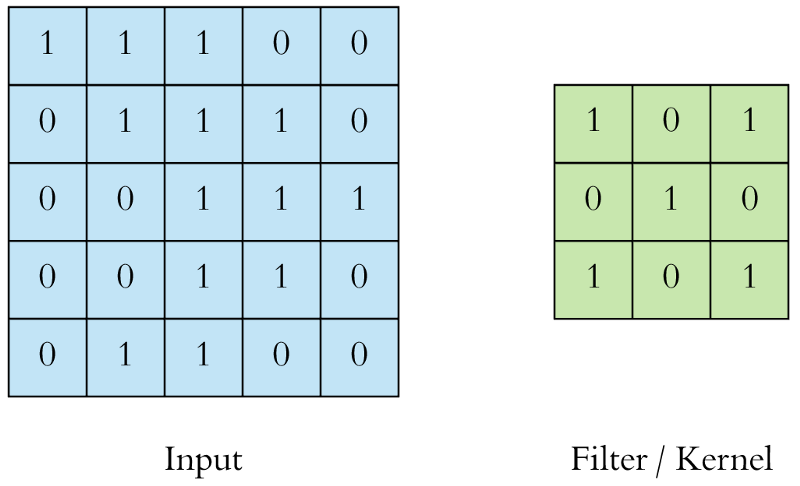
\includegraphics[scale=0.5]{Image/Convolution_input}
\end{center}

\bigskip

\textbf{Kết quả}
\begin{center}
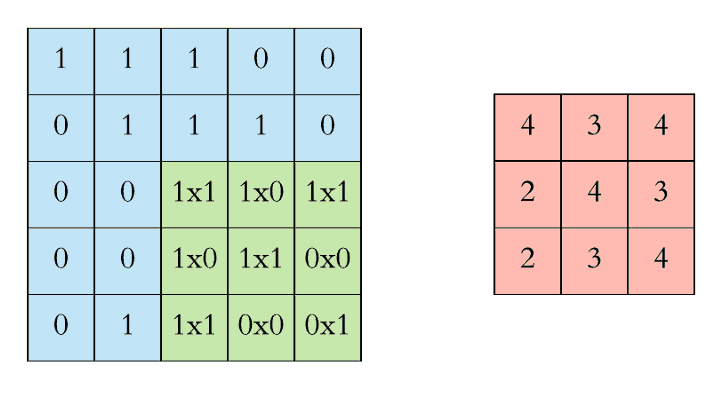
\includegraphics[scale=0.6]{Image/Convolution_res}
\end{center}

\subsubsection{Pooling}
Mục đích của \textbf{pooling} là làm giảm số chiều của ma trận, từ đó giảm thời gian tính toán và còn tránh được overfit.

Kiểu \textbf{pooling} được sử dụng phổ biến nhất là \textbf{max pooling} với từng ô $2*2$

\begin{center}
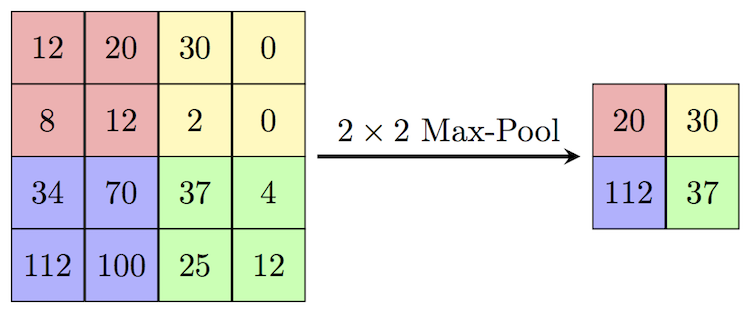
\includegraphics[scale=2]{Image/MaxpoolSample2}
\end{center}


\subsection{MT-CNN}
\textbf{MT-CNN} là mô hình mạng \textbf{neural} phát triển từ \textbf{CNN}. Mô hình này hoạt động rất mạnh trong việc nhận diện khuôn mặt. Đặc trưng của nó là dùng tăng độ chính xác cho việc nhận diện mặt bằng cách nhận diện thêm năm điểm đặc trưng trên khuôn mặt bao gồm: hai mắt, mũi và hai khóe miệng.

Kiến trúc của mạng \textbf{MT-CNN} là dùng lần lượt ba mô hình P-net, O-net, R-net.

\begin{center}
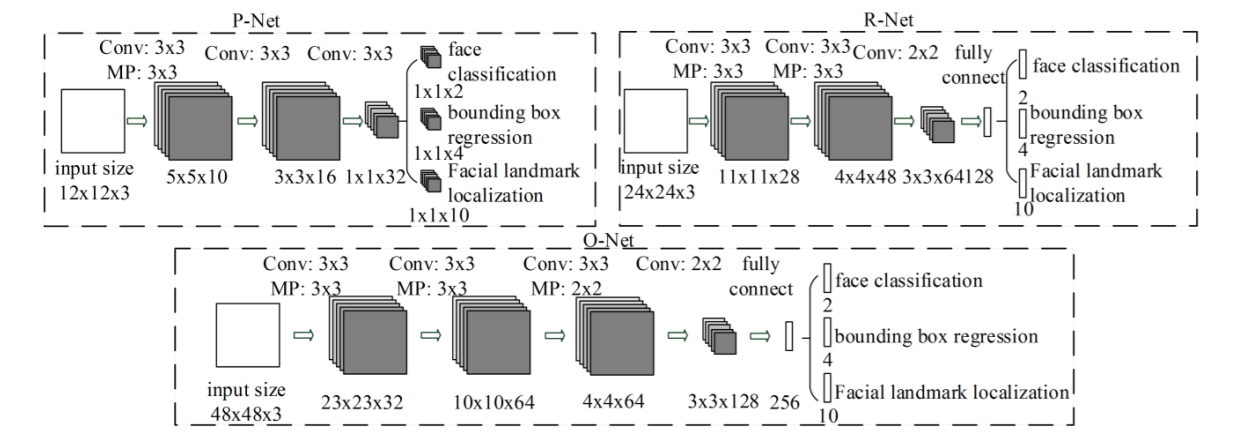
\includegraphics[scale=0.4]{Image/MTCNN_architecture}
\end{center}

\newpage
\subsubsection{P-net}
Tại P-Net, thuật toán sử dụng 1 kernel 12x12 chạy qua mỗi bức hình để tìm kiếm khuôn mặt.

\begin{center}
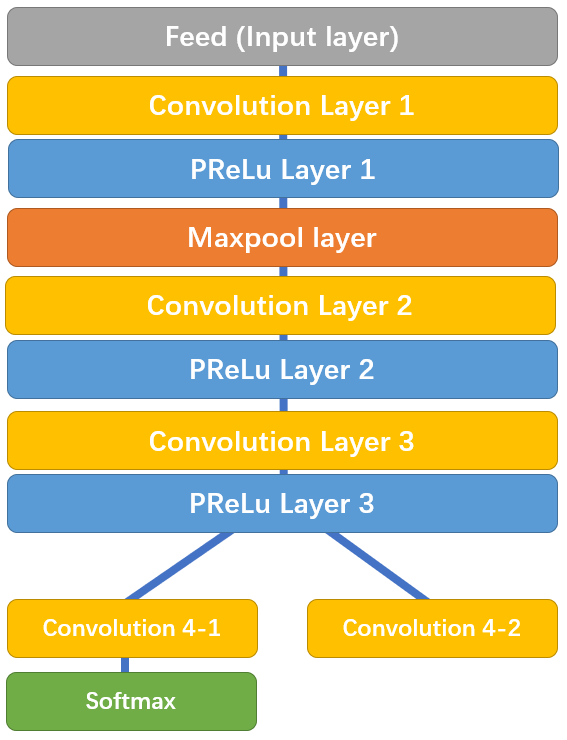
\includegraphics[scale=0.5]{Image/MTCNN_P_net}
\end{center}

Sau lớp convolution thứ 3, mạng chia thành 2 lớp. Convolution 4-1 đưa ra xác suất của một khuôn mặt nằm trong mỗi bounding boxes, và Convolution 4-2 cung cấp tọa độ của các bounding boxes. Đến đây, ta đã có cơ bản các \textbf{bounding box} có xác suất cao là chứa khuôn mặt.

\newpage
\subsubsection{R-net}
R-Net có cấu trúc tương tự với P-Net. Tuy nhiên sử dụng nhiều layer hơn. Tại đây, network sẽ sử dụng các bounding boxes đc cung cấp từ P-Net và tinh chỉnh là tọa độ.

\begin{center}
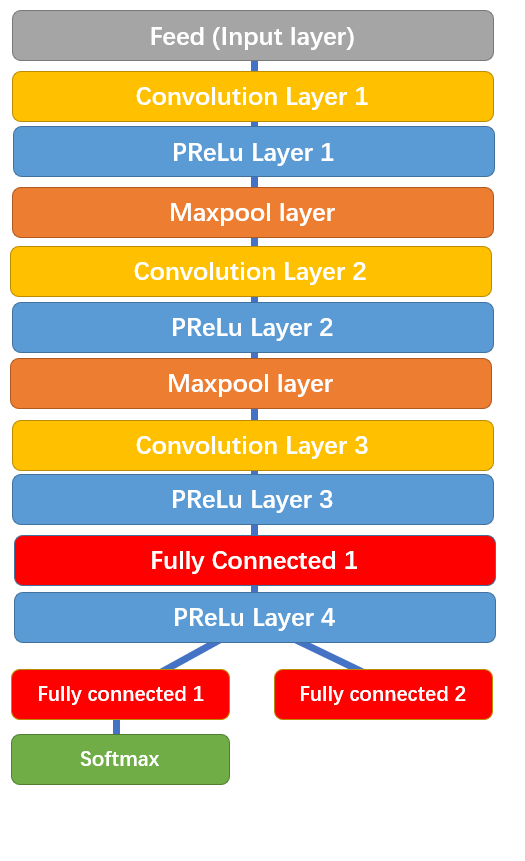
\includegraphics[scale=0.5]{Image/MTCNN_R_net}
\end{center}

Tương tự R-Net chia ra làm 2 layers ở bước cuối,cung cấp 2 đầu ra đó là tọa độ mới của các bounding boxes, cùng độ tin tưởng của nó.

\newpage
\subsubsection{O-net}
O-Net lấy các bounding boxes từ R-Net làm đầu vào và đánh dấu các tọa độ của các mốc trên khuôn mặt.

\begin{center}
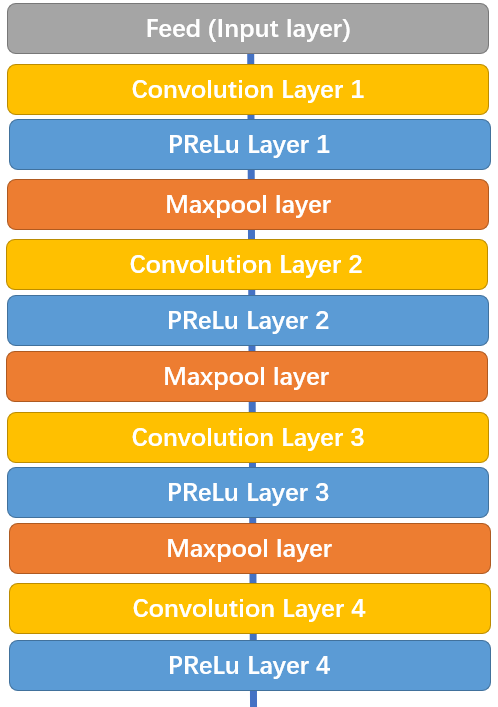
\includegraphics[scale=0.5]{Image/MTCNN_O_net}
\end{center}

\newpage

Ở bước này, thuật toán đưa ra 3 kết quả đầu ra khác nhau bao gồm: xác suất của khuôn mặt nằm trong bounding box, tọa độ của bounding box và tọa độ của các mốc trên khuôn mặt (vị trí mắt, mũi, miệng).

\begin{center}
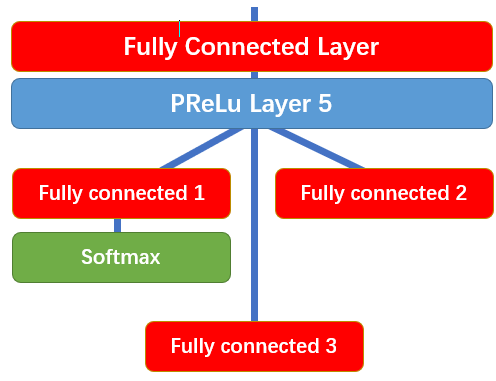
\includegraphics[scale=0.5]{Image/MTCNN_O_net_last}
\end{center}

\section{Recognize face}
Đầu vào của recognize là ma trận ảnh khuôn mặt được lấy từ phần nhận diện khuôn mặt. Ma trận ảnh này sẽ qua mô hình mạng \textbf{Inception ResNet v1} để được một vector đặc trưng với số chiều cố định. Sau đó, ta so khớp vector này với các vector đặc trưng đã được ghi sẵn trong cơ sở dữ liệu để cho ra kết quả.

\subsection{Inception Resnet v1}
\textbf{Inception Resnet v1} là mô hình mạng CNN phát triển. Đặc trưng của mô hình là phát triển theo chiều rộng. Tức là ở những tầng đặc biệt, ta sẽ dùng nhiều \textbf{filter} để kết hợp lại.

\begin{center}
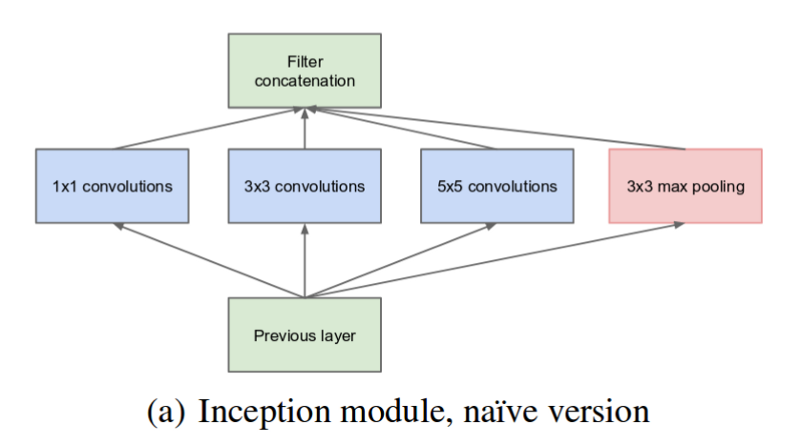
\includegraphics[scale=0.5]{Image/Inception_basic_1}

\bigskip

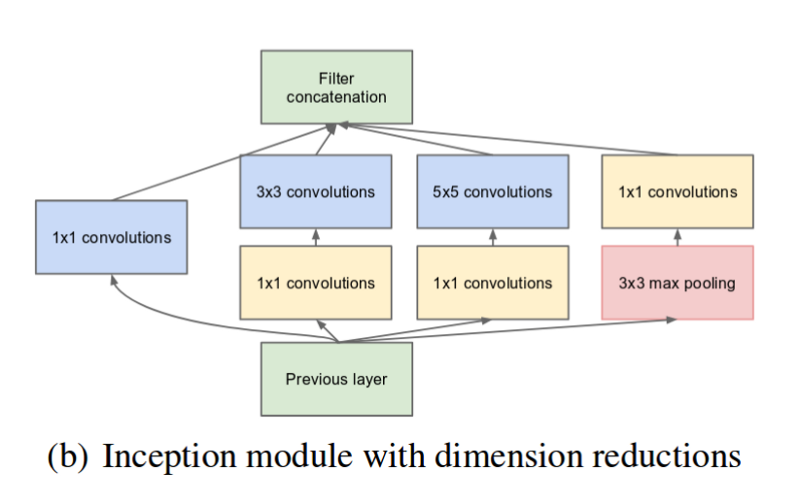
\includegraphics[scale=0.5]{Image/Inception_basic_2}
\end{center}

\newpage
\textit{VD:}
\begin{center}
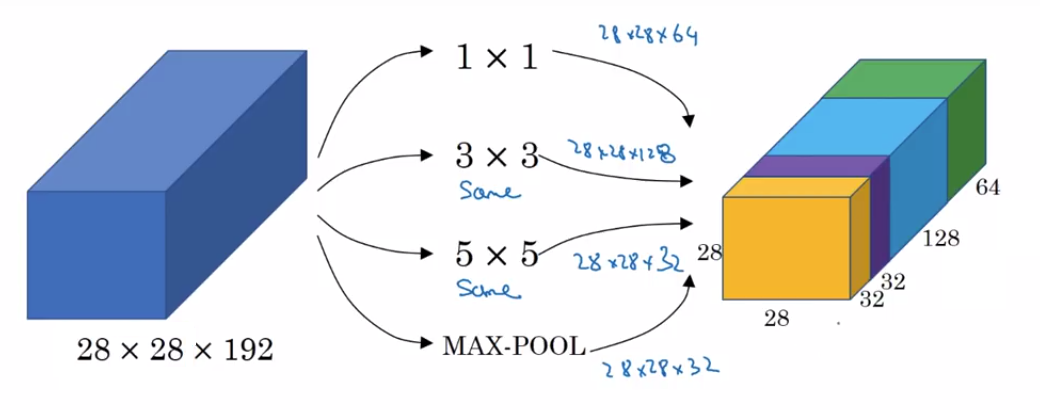
\includegraphics[scale=0.65]{Image/Inception_basic_example}

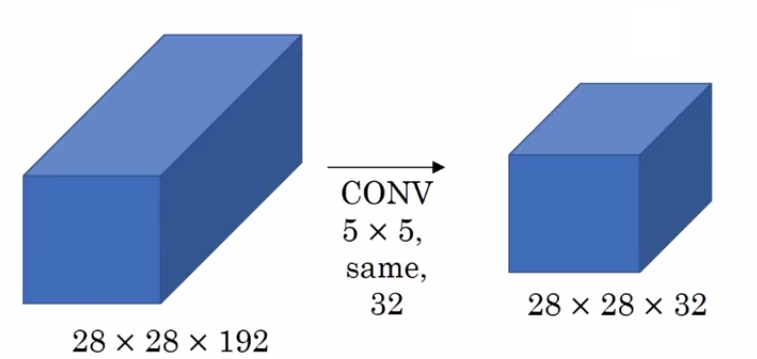
\includegraphics[scale=0.65]{Image/Inception_basic_example_1}
\end{center}

\subsubsection{Kiến trúc Inception Resnet v1}




\chapter{Kết quả}
\newpage
\chapter{Kết luận}
aaa

\newpage
\begin{thebibliography}{12}
	\addcontentsline{toc}{chapter}{\quad\  \bf Tài liệu tham khảo}
	\bibitem{1}On Certain Formal Properties of Grammars\\
	\textit{Noam Chomsky. In Information and Control 2, page 137 - 167, 1959.}
	\bibitem{2} Otomat và ngôn ngữ hình thức\\
	\textit{Đoàn Văn Ban, Bộ môn Khoa học máy tính, Khoa Công nghệ thông tin, Đại học Thái Nguyên.}
	\bibitem{3}Introduction to the Theory of Computation\\
	\textit{Michael Sipser. Cengage Learning, Boston, third edtion, 2013.
	}
	\bibitem{4}A Second Course in Formal Language\\
	\textit{Jeffrey Shallit. Cambridge University Press, 2009.}
	
	
	
\end{thebibliography}

\end{document}